\section{Background}

\subsection{Magnetic Resonance Imaging}

\ac{MRI} methods, such as T1 and T2 weighted imaging, measure the relaxation of a tissue's net magnetization vector. \cite{t1} These volumetric imaging methods are useful for distinguishing between different tissue types.\par
T1 relaxation time, also known as longitudinal relaxation time, refers to the time it takes for the protons to realign with the magnetic field after the radiofrequency pulse is turned off. Tissues with high-fat content, such as white matter in the brain, have shorter T1 relaxation times, which is why they appear bright on T1 weighted images. \cite{t1t2}\par
T2 relaxation time, also known as transverse relaxation time, measures how long it takes for protons to lose phase coherence among the spins perpendicular to the magnetic field. This is influenced by the interaction of spins within the tissue. Tissues with high water content, like cerebrospinal fluid, have longer T2 relaxation times, appearing bright on T2 weighted images. \cite{t1t2}\par

Neurons, the electrically excitable cells of the brain, process and transmit information via electro-chemical signaling. \cite{brain} The main function of the white matter is to connect neurons from different brain regions to each other by myelinated nerve fibers. \cite{white} The myelin sheath is a greatly extended and modified plasma membrane wrapped around the nerve axon. \cite{myelin}\par

\ac{DTI} is a specialized \ac{MRI} technique that measures the rate and direction of movement of water molecules within tissues. In the \ac{CNS}, axonal tracts and myelin present physical barriers that impose directionality or anisotropy on water diffusion (\reflink{fig:dti}{Figure} from \cite{dti}). Applying magnetic field gradients allows the measurement of the rate and direction of the movement of water molecules in the direction of the magnetic field. Using the basis of diffusion, we can construct a 3D directional architecture of axon fibers and myelin in the \ac{CNS}. \cite{dti}
\begin{figure}[H]
\centering
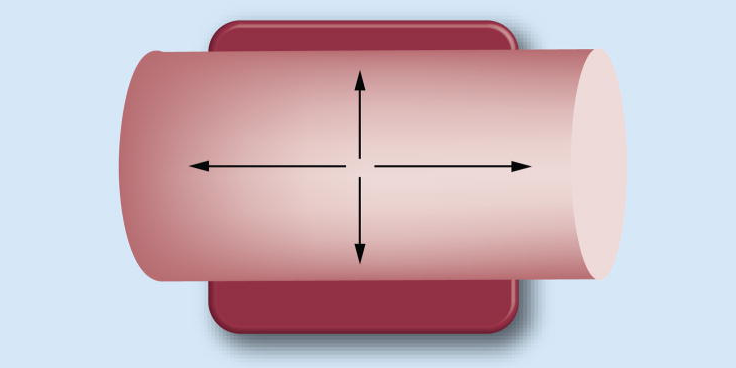
\includegraphics[width=0.4\textwidth]{dti0}
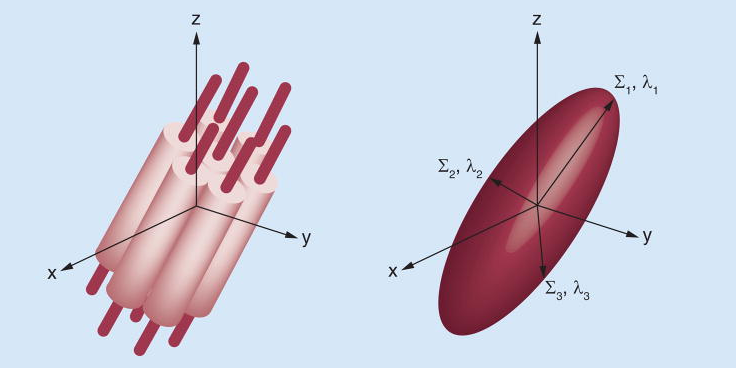
\includegraphics[width=0.4\textwidth]{dti1}
\caption{Physical Barrier Restricting Diffusion in \acs{DTI}}
\label{fig:dti}
\end{figure}
Certain images extracted from a \ac{DTI} image, like \ac{FA} and \ac{MD} are invaluable for characterizing, researching and diagnosing neurodegenerative diseases. The \ac{FA} scalar measures the fraction of the diffusion, where an isotropic medium takes a value of 0 and a cylindrically symmetric anisotropic medium takes a value of 1. The \ac{MD} scalar measures how freely water molecules move in tissue, where greater tissue density means lower \ac{MD}. \cite{rd}\par
Furthermore, a more complicated algorithm can be employed to extract information regarding the connectivity of brain regions, specifically using tractography methods to model the trajectories of white matter pathways. Tractography algorithms, such as probabilistic tractography, can simulate numerous potential pathways (tracts) originating from a seed region. These tracts can be traced to determine their likelihood of reaching specific target regions. Each voxel within the seed region can be assigned a connectivity value based on the proportion of simulated tracts that successfully reach a given target region, providing a probabilistic measure of connectivity. Once these connectivity values are obtained, the seed region can be segmented, or parcellated, into distinct subregions that are preferentially connected to different targets. This connectivity based parcellation enables a detailed examination of the structural organization of brain regions and their relationship with target areas, contributing valuable insights into both healthy and pathological brain networks. \cite{tract} \cite{tract2}\par
However, due to \ac{DTI} not being part of many clinical protocols, and it taking a relatively long time to acquire, it is not widely available in actual practice.

\subsection{Radiomics}

Although the term is not strictly defined, radiomics generally refers to the extraction of quantitative, and ideally reproducible, information from diagnostic images, including complex patterns that are difficult to recognize or quantify by the human eye. \cite{radio} Radiomic features capture tissue characteristics such as heterogeneity, shape, texture, intensity, spatial relationships, edge sharpness, contrast and much more. \cite{radio2} Radiomic features can be extracted using voxel-based and non-voxel-based approaches. A voxel is the atomic element of a volumetric image, such as an MRI record (analogous to a pixel in a 2D image). In the voxel-based method, features are derived from each voxel and its surrounding area using a kernel-based approach similar to convolution. Conversely, the non-voxel-based method extracts features from any arbitrary mask used as a kernel, which could encompass specific regions or even the entire brain.

\subsection{Basal Ganglia and Huntington’s Disease}

Basal ganglia is a part of the human brain which is a group of subcortical nuclei responsible primarily for motor control, as well as other roles such as motor learning, executive functions and behaviors, and emotions. \cite{basal} \ac{HD} is a disorder that causes the progressive degeneration of the basal nuclei. \cite{hunting} This manifests as both structural connectivity changes and anatomical volume changes. \cite{basal2}\par

\section{State of the Art}
\label{sec:stateoftheart}

Several state-of-the-art studies form the foundation of this project. Research has shown that the ratio of commonly acquired T1 and T2 weighted images can serve as a proxy for myelin content. This suggests that structural connectivity information can be indirectly derived from these anatomical scans. For instance, one study \cite{myelin2} successfully mapped myelin content in the brain using the T1/T2 ratio. Similarly, another study \cite{myelin} utilized this ratio to delineate cortical areas of the brain based on myelin distribution. Additionally, \cite{myelin3} identified direct correlations between the \ac{MWF} and the T1/T2 ratio.\par
Machine learning has also become increasingly prominent in medical imaging, particularly in tumor segmentation. Architectures like U-Net, a type of \ac{FCNN}, have proven highly effective in this domain. Numerous studies, such as \cite{unetseg} \cite{unetseg2} \cite{unetseg3} \cite{unetseg4} \cite{unetseg5} (and many more), employ solutions built on similar architectures. However, most of these methods operate on 2D slices of 3D volumes, as 2D convolutional backbones are better explored and computationally more efficient, avoiding the exponential increase in resource demands associated with higher dimensions.\par
Another widely used technique in medical image analysis is radiomics, which offers a deterministic approach to feature extraction. This method facilitates the identification of image-derived biomarkers that can be correlated with specific clinical labels, such as tumor segmentation. \cite{radioseg} \cite{radioseg2} \cite{radioseg3} A key advantage of radiomics is that, unlike \ac{NN}-based methods, it can efficiently operate on 3D volumes without the significantly higher computational demands that often render 3D neural networks less feasible in practice.

\section{Motivation}

The state-of-the-art studies highlight an intriguing possibility: can structural connectivity images be synthesized directly from anatomical T1 and T2 weighted images using machine learning? Such a development could bypass the time and resource intensive processes associated with \ac{DTI} acquisition and post processing, such as tractography. Furthermore, it would allow the synthesis of these less commonly available images from historical datasets that often only include anatomical scans, greatly enhancing their utility in retrospective analyses.\par
\ac{FCNN} and radiomics based approaches have demonstrated exceptional accuracy in tasks like tumor segmentation, showcasing their potential for high-precision medical imaging applications. However, surprisingly few studies have explored synthesizing \ac{DTI} related images from T1 and T2 data. Moreover, the integration of radiomics with \ac{NN}-based methods remains underexplored, despite the complementary nature of these techniques. Radiomic features, extracted voxel based from 3D volumes, are conceptually parallel the feature extraction role of \ac{CNN} backbones, but offer unique advantages in handling 3D data.\par
By combining radiomics with \ac{NN}s, a hybrid approach could capitalize on the strengths of both paradigms. Specifically, appending a \ac{NN} head for classification or regression to voxel based radiomic features would enable the use of truly 3D information without incurring the significant computational overhead associated with 3D \ac{CNN}s. This hybrid strategy could pave the way for efficient and accurate synthesis of structural connectivity images, leveraging the elasticity of \ac{NN}s while retaining the richness of 3D volumetric features.

\section{Objectives}

The primary objective of this research is to integrate radiomics based feature extraction with \ac{NN}s to predict \ac{FA}, \ac{MD}, and relative connectivity from T1 and T2 weighted images. The study aims to explore voxel based features, potentially in combination with non voxel based features extracted from several cortical areas. Since the feature extraction process relies on non \ac{NN} techniques, the classification or regression head will utilize a \ac{FNN}, akin to the fully connected layers of a \ac{CNN} following the flattening of convolutional layers.\par
Additionally, this work will assess the robustness of the proposed method by conducting experiments on datasets containing healthy control participants and those affected by \ac{HD} neurodegeneration, through separating or combining the two groups.\par
The scope of this project has been intentionally narrowed to ensure its feasibility within the timeframe of the thesis. Specifically, the research focuses on the basal ganglia as the primary \ac{ROI}. This decision allows for a concentrated examination of a well defined brain area closely associated with structural and functional connectivity, while managing the computational and methodological demands of the study.\par
Additionally, the study is designed as a simplified proof of concept, utilizing a limited dataset. This constraint reflects the exploratory nature of the work, aiming to establish the feasibility of synthesizing structural connectivity images from T1 and T2 weighted scans using the proposed methodology. The results are therefore not intended to represent a generalized or universally applicable solution but rather to demonstrate the potential of this approach for future, more expansive investigations.\par
It is important to note that this research does not aim to cover the full spectrum of structural connectivity imaging across the brain or account for variations introduced by diverse pathological or demographic factors. Instead, the findings are expected to provide a foundation for subsequent studies that can explore broader generalizability, larger datasets, and more comprehensive analyses of multiple brain regions. These limitations should be considered when interpreting the results and their potential applications.

\subsection{Previous Work}

Detailed data acquisition, pre and post processing steps of the previous work done at Hospital de Bellvitge (L'Hospitalet de Llobregat, Barcelona, Spain) are detailed in \reflink{sec:previous}{Appendix}. In summary, Hospital de Bellvitge provided an excellent dataset of anatomocal \ac{MRI} and \ac{DTI} records of 32 control and 38 \ac{HD} patient records of T1 and T1/T2 \ac{MRI} images with isotropic voxels of 1 millimeter resolution and \ac{DTI} \ac{FA} and \ac{MD} images with isotropic voxels of 2 millimeter resolution. Furthermore this dataset also contains the mask for the basal ganglia, which will also be referenced as the \ac{ROI}; masks for the 7 cortical regions of the brain, which will also be referenced as the target regions: Limbic, Executive, Rostral-Motor, Caudal-Motor, Parietal, Occipital and Temporal; streamline images and relative connectivity maps from the results of tractography; subcortical segmentation of the basal ganglia for the Caudate, Putamen and Accumbens; and \ac{FNIRT} warp fields for converting the records into normalized space.\par
Furthermore, for both the \ac{ROI} and cortical targets, the dataset distinguishes between the right and left hemispheres of the brain. Thus there are actually 2 \ac{ROI}s and $2 \cdot 7=14$ target regions.

